\chapter{Particle Flow Calorimetry for Future Linear Colliders}
\label{chap:pflowandlcdetectors}

\chapterquote{I am fond of pigs.  Dogs look up to us.  Cats look down on us.  Pigs treat us as equals.}
{Winston Churchill}

%========================================================================================
%========================================================================================

Particle flow calorimetry can provide extremely good jet energy resolutions for at a future linear collider.  Jet energy resolution is crucial at the linear collider as many of the interesting processes will be characterised by multi-jet final states.  Many of these multi-jet final states will be produced from the hadronic decays of W and Z bosons and one of the key goals of the future linear collider is to be able to separate these decays.  Separation of these decays can be achieved, however, only by placing a tight requirement on the jet energy resolution; $\sigma_{E}/E \lessapprox 3.5\%$ for 50-500~GeV jets at the ILC and up to 1.5~TeV at CLIC \cite{arXiv:0907.3577}.  The use of particle flow calorimetry will also be highly beneficial for quantifying final states of interest that involving charged leptons and missing momentum.  

%========================================================================================
%========================================================================================

\section{Particle Flow Calorimetry}
The premise of particle flow calorimetry is to use the sub-detector that offers the best energy resolution to measure the energy of any given particle, which corresponds to energy measurements being made in the ECal for $\gamma$s, the HCal for neutral hadrons and, crucially, the tracker for charged particles.  The starkest contrast of this approach to that of traditional calorimetry occurs in the measurement of the energy of charged particles.  In particle flow calorimetry the energy of a charged particle is measured using the curvature of the path it transverses as it bends in a magnetic field, while in traditional calorimetry the energy would be measured using the calorimeters, predominantly the hadronic calorimeter (HCal).  The tracker energy resolution for a single charged particle of energy $E_{X^{\pm}}$ is $\sim 10^{-4} \times E_{X^{\pm}}^{2}$, while for the HCal it is $\sim 0.55 \times \sqrt{E_{X^{\pm}}}$ \cite{arXiv:0907.3577}.  The energy resolution offered by the tracker is significantly better than that offered by the HCal for energies up to $\sim \mathcal{O}(300 \text{ GeV})$.  This means that particle flow calorimetry has the potential to offer a much better energy resolution for charged particles, below $\sim \mathcal{O}(300 \text{ GeV})$, than that of the traditional calorimetry approach.  Particle flow calorimetry offers gains in performance for collision energies well beyond 300 GeV as the average long-lived particle energy for physics processes of interest is typically much less than 300 GeV.  Furthermore, it also leads to a significant improvement in the measurement of jet energies as, after the decay of short-lived particles, approximately 60\% of the energy of a jet is carried in the form of charged particles.  The measurement of jet energies in the particle flow paradigm is summarised in table \ref{table:pflowjet}.  The benefits to the energy resolution, for both charged particles and jets, offered by the particle flow approach to calorimetry is the driving factor behind why it is planned for used at the linear collider experiment.  

\begin{table}[h!]
\centering
\begin{tabular}{ l l l l l}
\hline
Jet  & Detector & Energy & Energy\\
Component &  & Fraction & Resolution\\
\hline
Charged Particles ($X^{\pm}$) & Tracker & $\sim 0.6 E_{j}$ & $10^{-4} \times E_{X^{\pm}}^{2}$ \\
Photons ($\gamma$) & ECal & $\sim 0.3 E_{j}$ & $0.15 \times \sqrt{E_{\gamma}}$ \\
Neutral Hadrons ($X^{0}$) & HCal &$\sim 0.1 E_{j}$ & $0.55 \times \sqrt{E_{X^{0}}}$ \\
\hline
\end{tabular}
\caption[The approximate jet fractions and energy resolutions for charged particles ($X^{\pm}$) of energy $E_{X^{\pm}}$, photons ($\gamma$) of energy $E_{\gamma}$ and neutral hadrons ($X^{0}$) of energy $E_{X^{0}}$.  Taken from \cite{arXiv:0907.3577}.]{The approximate jet fractions and energy resolutions for charged particles ($X^{\pm}$) of energy $E_{X^{\pm}}$, photons ($\gamma$) of energy $E_{\gamma}$ and neutral hadrons ($X^{0}$) of energy $E_{X^{0}}$.  Taken from \cite{arXiv:0907.3577}.}
\label{table:pflowjet}
\end{table}

Particle flow calorimetry is challenging to put into practice as it requires a precise reconstruction for all long-lived particles within a detector.  Charged particle energy measurements are made using the curvature of the track they transverse as they bend in the magnetic field, but they also produce calorimetric energy deposits, as shown in figure \ref{fig:particleflowpic}.  If both energy measurements are included the energy of the charged particle will be double counted.  To avoid this, any calorimetric energy deposits associated to charged particle tracks are not used when reporting the reconstructed energy.  However, this means that if the calorimetric energy deposits for a neutral particle are incorrectly associated to a track, the energy measurement for that neutral particle will be totally omitted.  The combination of this double counting of charged particle energies and loss of neutral particle energies form the confusion contribution to the jet energy resolution, which acts to degrade the energy resolution.  Particle flow calorimetry hinges on the event reconstruction being able to correctly associate all charged particle tracks to their corresponding calorimetric energy deposits.  This can only be realised by using calorimeters with fine segmentation so that it is possible to resolve individual particle showers within them coupled with sophisticated pattern recognition algorithms to reduce the effects of confusion.

\begin{figure}[h!]
\centering
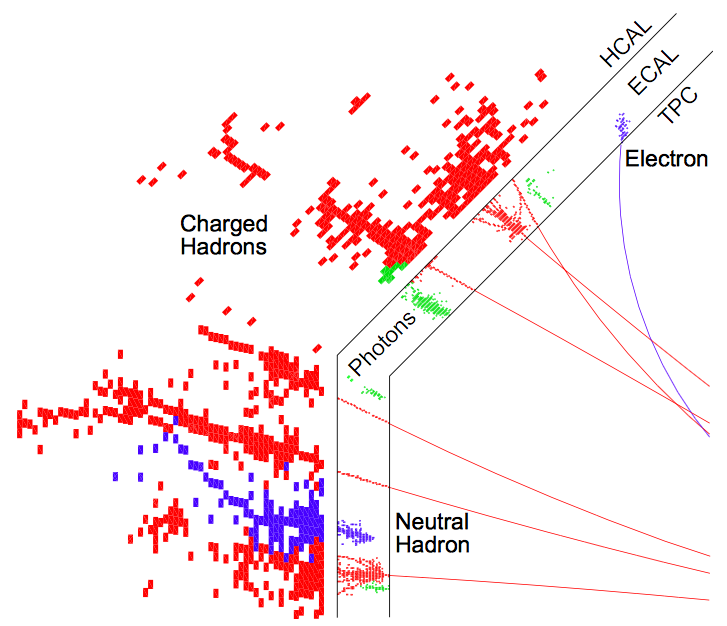
\includegraphics[width=0.5\textwidth]{LCDetectorsAndPFlow/Plots/Pictures/PFlow.png}
\caption[A typical simulated 250 GeV jet in the CLIC\_ILD detector, with labels identifying constituent particles.  Image taken from  \cite{arXiv:1209.4039}.]{A typical simulated 250 GeV jet in the CLIC\_ILD detector, with labels identifying constituent particles.  Image taken from  \cite{arXiv:1209.4039}.}
\label{fig:particleflowpic}
\end{figure} 

%========================================================================================
%========================================================================================

\section{International Large Detector}
\label{sec:ild}

%========================================================================================

\subsection{Overview}
All detector concepts for the linear collider have been purposely built to make particle flow calorimetry possible.  While there are a number of different concepts that are under consideration for both the ILC and CLIC one of the most prominent, and the focus of this work, is the International Large Detector (ILD).  The ILD detector, shown in figure \ref{fig:ild} achieves very high spatial resolution for all sub-detector systems thanks to its highly segmented calorimeters and central tracking system, both of which are encompassed within a 3.5 T magnetic field.  When combined with sophisticated pattern recognition software, provided by PandoraPFA, particle flow calorimetry can be realised and the linear collider jet energy resolution goal of $3.8 \%$, which is required to allow separation of hadronic decays from W and Z bosons, can be achieved.

\begin{figure}[h!]
\centering
\subfloat[]{\label{fig:ild1}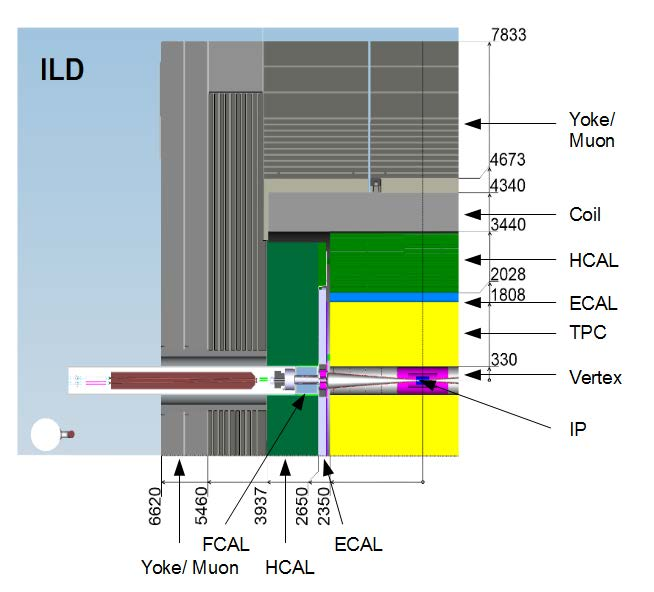
\includegraphics[width=0.5\textwidth]{LCDetectorsAndPFlow/Plots/Pictures/ILD.jpg}}
\subfloat[]{\label{fig:ild2}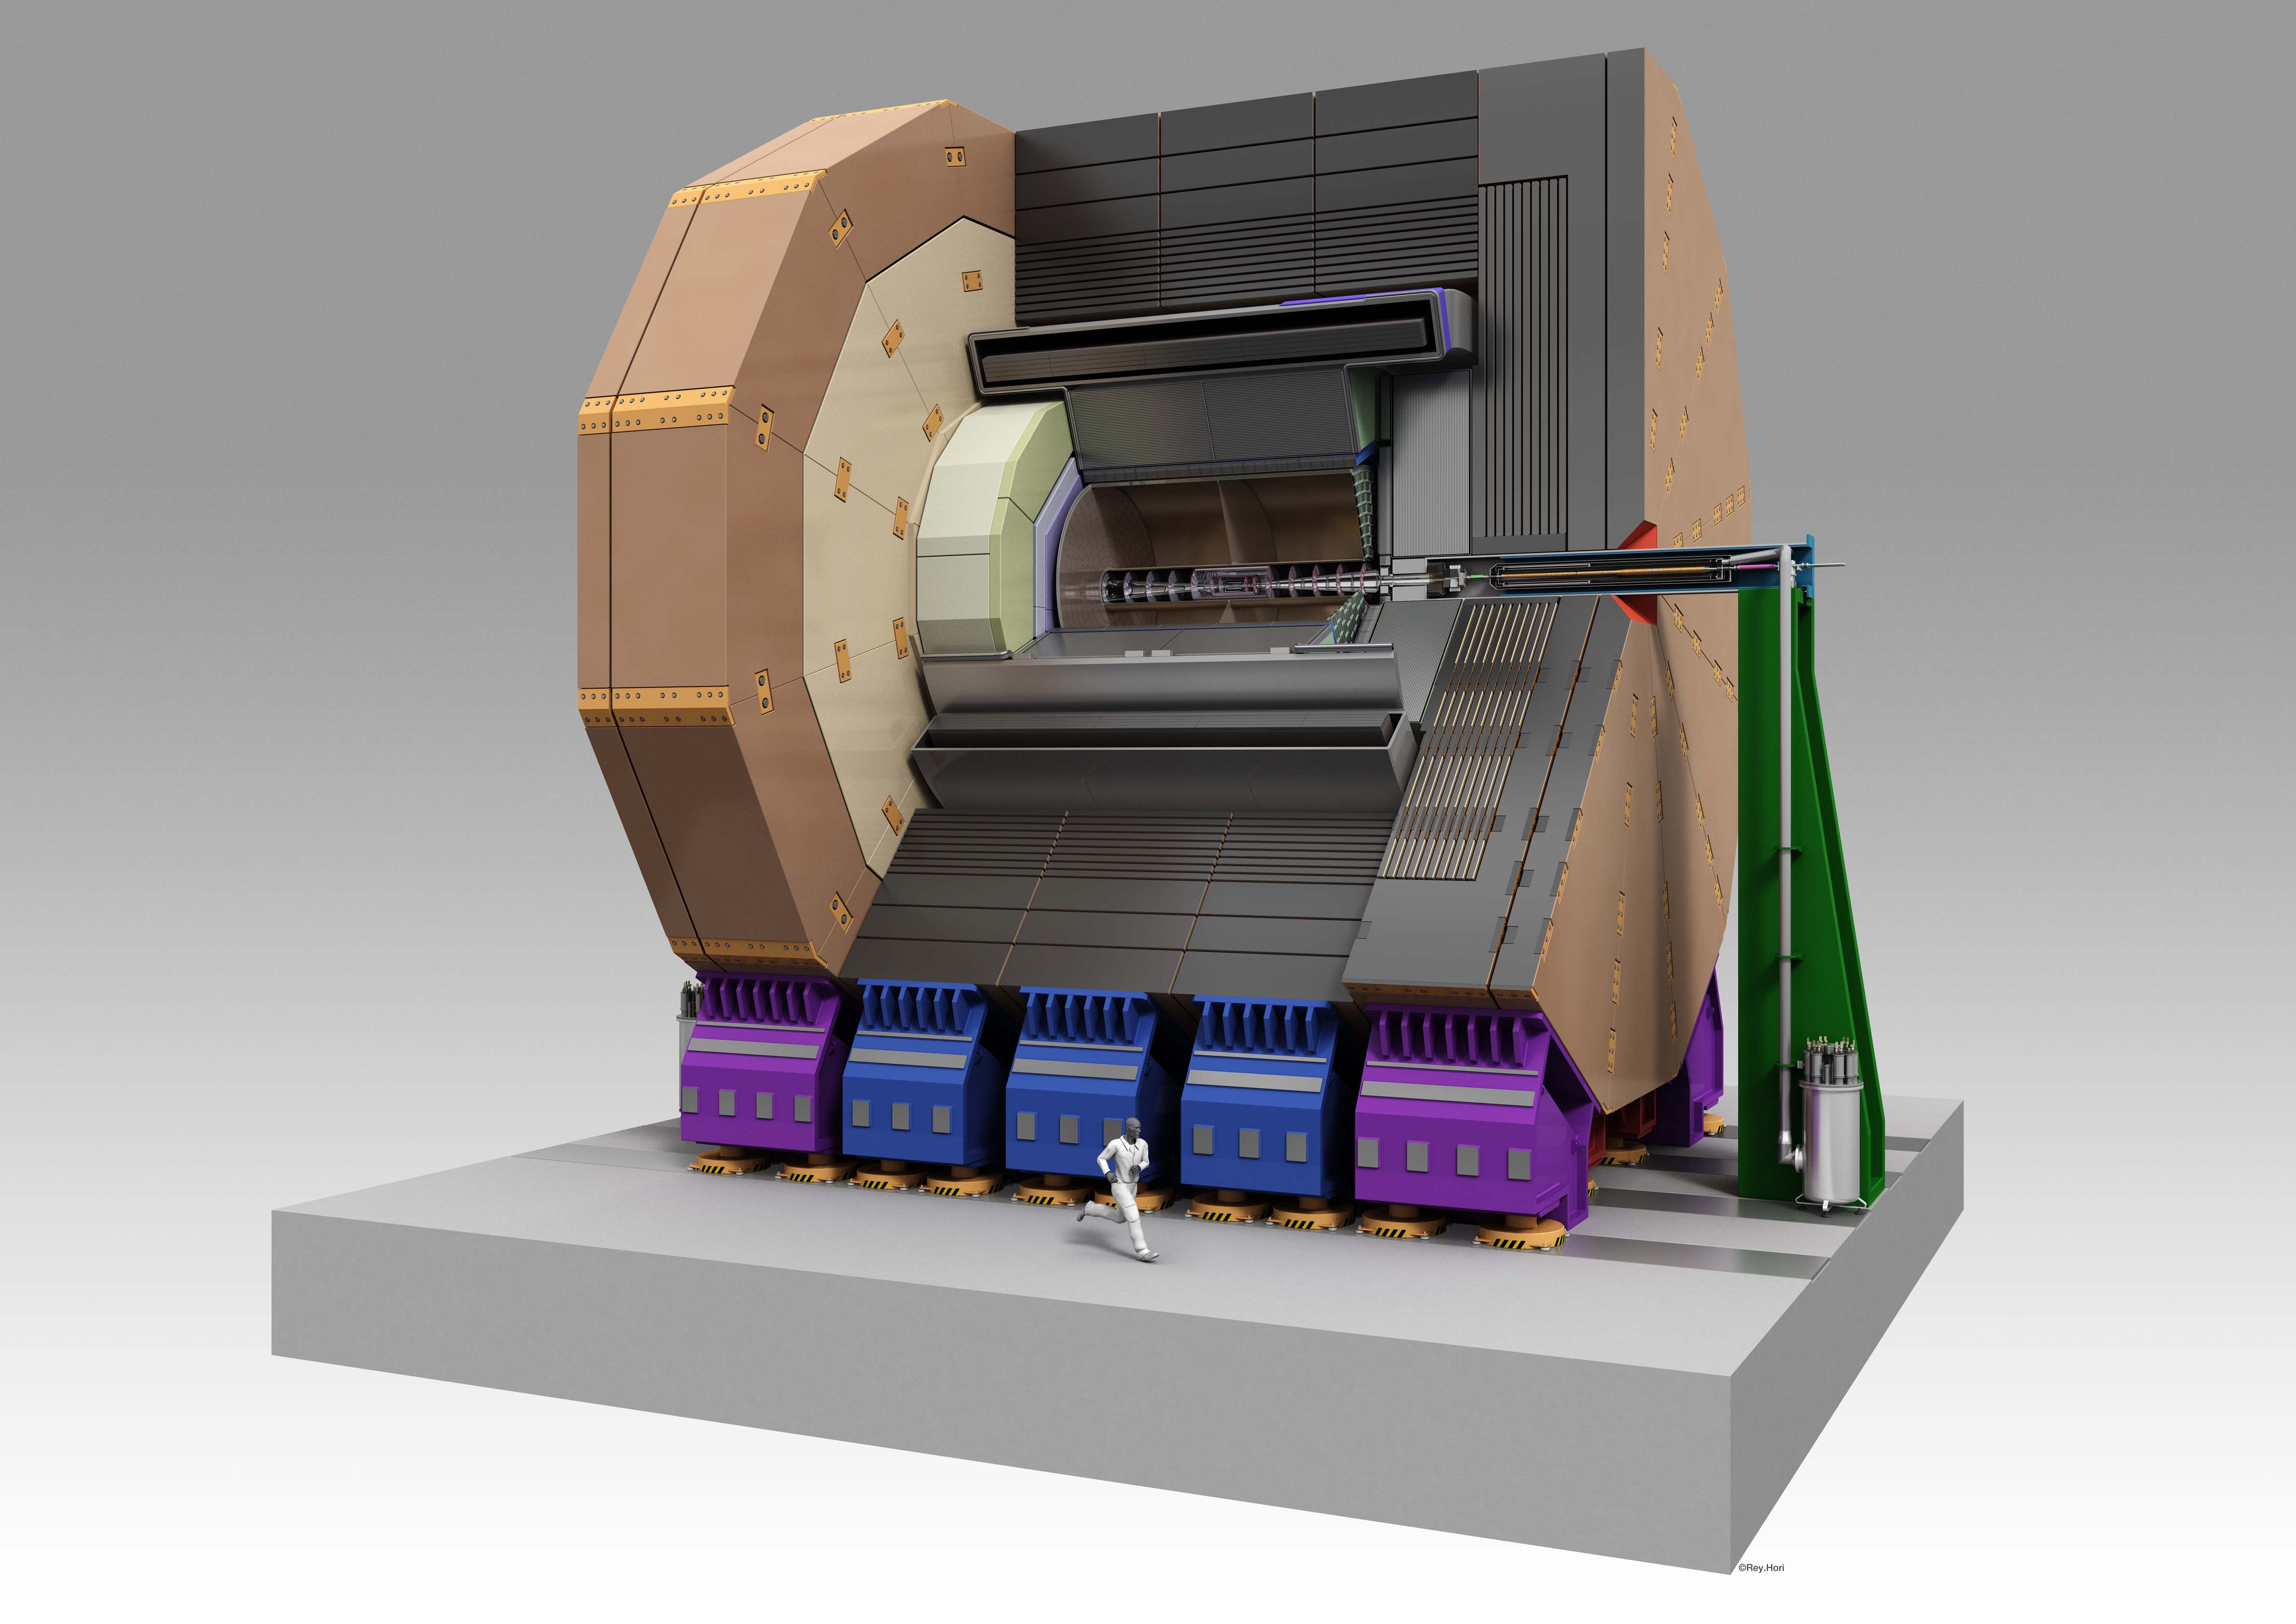
\includegraphics[width=0.5\textwidth]{LCDetectorsAndPFlow/Plots/Pictures/ILD_2.jpg}}
\caption[\protect\subref{fig:ild1} Quadrant view of the ILD detector concept.  The interaction point is in the lower right corner of the picture.  Dimensions are in mm.  \protect\subref{fig:ild2} View of the ILD detector concept.  Figures taken from  \cite{Behnke:2013lya}.]{\protect\subref{fig:ild1} Quadrant view of the ILD detector concept.  The interaction point is in the lower right corner of the picture.  Dimensions are in mm.  \protect\subref{fig:ild2} View of the ILD detector concept.  Figures taken from  \cite{Behnke:2013lya}.}
\label{fig:ild}
\end{figure} 

%========================================================================================

\subsection{Vertex Detector}
The tracking system for the ILD detector consist of a multi-layer pixel-vertex detector, which is surrounded by a system of silicon strip and pixel detectors.  These are designed to give precise information about displaced vertices with respect to the impact point, which are crucial for the study of short lived particles such as the $D$ or $B$ mesons.  Outside of the vertex detector is the central tracker of ILD, which is a Time Projection Chamber (TPC).  The TPC samples each charged particle track at many points giving detailed spatial information that can be used to extract the curvature of the track and hence the momentum of the charged particle that transversed it.  Finally, a further silicon strip detector surrounds the TPC to give an additional, high precision, space point to aid tracking performance. 


The main goal of the ILD vertex detector is to achieve a resolution on the impact parameter of charged particle tracks of $\sigma_{b} < 5 \oplus \frac{10}{p\text{sin}(\theta)^{3/2}} \mu$m, where the first term is the transverse impact parameters resolution and the second is a multiple-scattering term.  This makes precisely tagging secondary vertices from charm and bottom mesons possible.  Typically these mesons have relatively short proper lifetimes, $\tau$, such that $c\tau \approx \mathcal{O}(300 \text{{\mu}m})$.  To achieve this impact parameter resolution, a spatial resolution of better than 3 {\mu}m is required near the IP.  Furthermore, a low material budget of less than 0.15 \% $X_{0}$ per layer is required to ensure that few electromagnetic showers are initiated within the vertex detector.  A low pixel occupancy is essential for determining the trajectory of individual tracks in the detector.  The vertex detector will also have to be radiation hard to cope with the intense beam induced backgrounds, which are predominantly from beamstrahlung, found close to the IP at the linear collider.  Furthermore, consideration will have to be given to the mechanical structure of the detector, power consumption and cooling.  

There are a number of different pixel technology options under consideration for the vertex detector for the ILD detector and this is an active area of ongoing research and development for the linear collider collaboration.  The current design of the vertex detector consists of three concentric layers of double-sided ladders that are close to being cylindrical.  Each ladder has two pixel sensors on each side and the ladder thickness is approximately 2 mm.  The inner most radii of the ladders ranges from 16 mm to 60mm from the IP.  In the simulation of the vertex detector silicon is used as the sensitive material.  Support material and a cryostat are also included in the simulation for further realism.  

%========================================================================================

\subsection{TPC}
The central tracking system for the ILD detector is a TPC, which is shown in figure \ref{fig:tracker}.  The TPC consists of two chambers of gas with a high voltage applied across them.  Charged particles passing through the TPC ionise the gas and the ionised molecules drift in the high voltage to the end plates where they are collected and measured.  The drift time is then used to calculate the position of the ionisation point.  TPCs have an advantage over silicon tracking in that they continuously track any charged particle passing through them, while silicon detectors are only sensitive within each silicon layer.  This compensates for the worse single point resolution that TPCs have in comparison to silicon detectors and makes TPCs a viable option for the ILD detector.  Furthermore, TPCs has a very low material budget, which benefits calorimetry in ILD.  

The ILD TPC will operate within a 3.5 T magnetic field and under these conditions a point resolution of better than 100 {\mu}m and a double hit resolution in $\phi$ of less than 2 mm can be achieved.  Several readout technology options are currently under development for the ILD TPC and each of these is tailored to the gas mixture that will be used for the TPC.  For all potential options it is envisaged that the readout pads would be $\approx 1 \times 6 \text{mm}^{2}$ giving a total of approximately $10^{6}$ on the TPC endplates.

In the detector simulation the TPC is simulated as a cylindrical volume of the gas mixture, Ar:$\text{CH}_4$:$CO_{2}$ (95:3:2) \cite{Abe:2010aa}, which is surrounded by a realistic field cage.  A conservative estimate of the endplate is included in the simulation to account for the support structure, electronics and cooling pipes for the TPC.  Furthermore, the material budget required to account for power and readout cables for the inner vertex detector has been estimated and is included in the simulation as an aluminium cylinder between the beam pipe and the field cage of the TPC.

\begin{figure}[h!]
\centering
\subfloat[]{\label{fig:tracker1}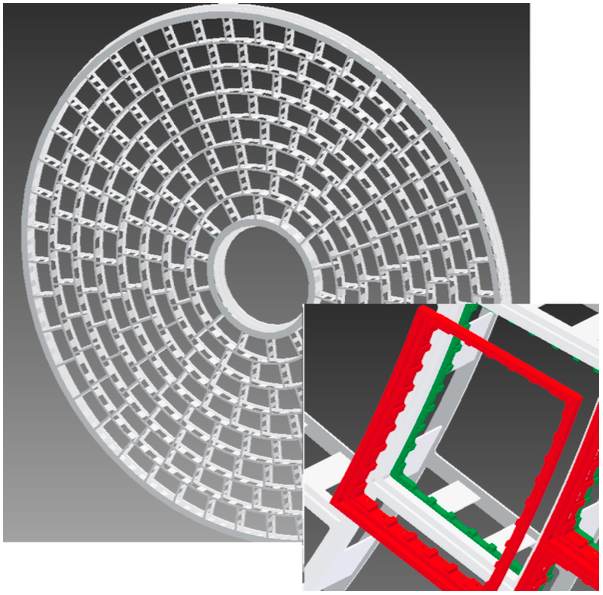
\includegraphics[width=0.5\textwidth]{LCDetectorsAndPFlow/Plots/Pictures/Tracker1.png}}
\subfloat[]{\label{fig:tracker2}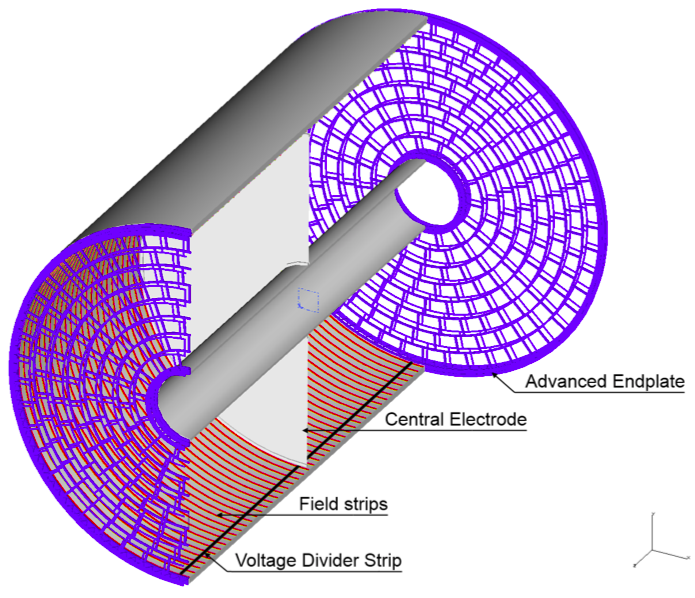
\includegraphics[width=0.5\textwidth]{LCDetectorsAndPFlow/Plots/Pictures/Tracker2.png}}
\caption[\protect\subref{fig:tracker1} Drawing of the propose end-plate for the TPC.  \protect\subref{fig:tracker2} Conceptual sketch of the TPC system showing the main parts of the TPC (not to scale).  Figures taken from  \cite{Behnke:2013lya}.]{\protect\subref{fig:tracker1} Drawing of the propose end-plate for the TPC.  \protect\subref{fig:tracker2} Conceptual sketch of the TPC system showing the main parts of the TPC (not to scale).  Figures taken from  \cite{Behnke:2013lya}.}
\label{fig:tracker}
\end{figure} 

%========================================================================================

\subsection{Supplemental Silicon Tracking System}
% Requires restructuring as moved TPC upfront 
There are four components that make up the silicon tracking system for ILD, shown in figure \ref{fig:vertex}, which are:

\begin{figure}[h!]
\centering
\subfloat[]{\label{fig:vertex1}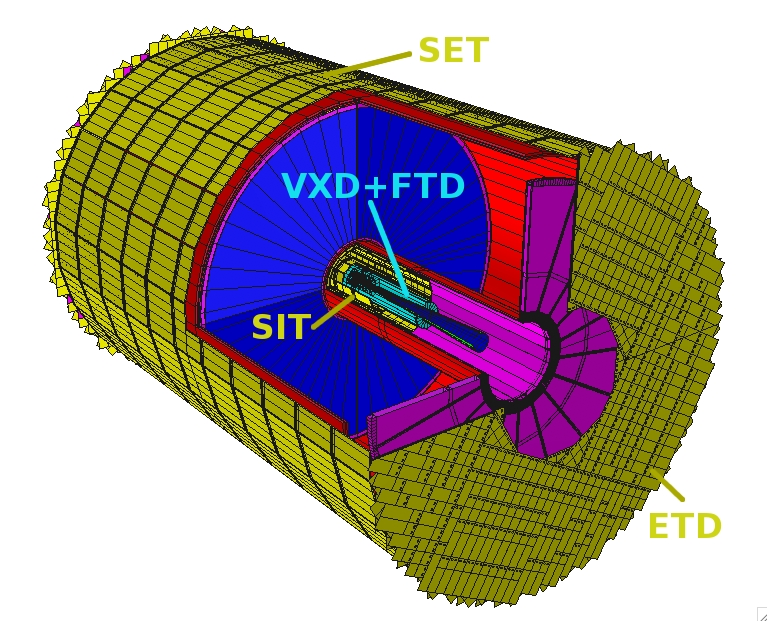
\includegraphics[width=0.5\textwidth]{LCDetectorsAndPFlow/Plots/Pictures/Vertex1.jpg}}
\subfloat[]{\label{fig:vertex2}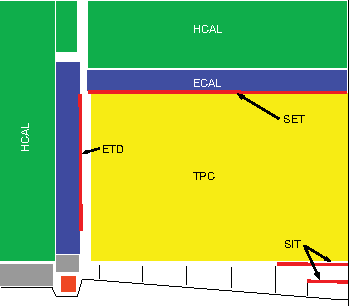
\includegraphics[width=0.5\textwidth]{LCDetectorsAndPFlow/Plots/Pictures/Vertex2.pdf}}
\caption[\protect\subref{fig:vertex1} A quadrant view of the ILD silicon envelope made of the four components SIT, SET, ETD and FTD as included in the full MOKKA simulation.  \protect\subref{fig:vertex2} a 3D detailed GEANT4 simulation description of the silicon system.  Figures taken from  \cite{Behnke:2013lya}.]{\protect\subref{fig:vertex1} A quadrant view of the ILD silicon envelope made of the four components SIT, SET, ETD and FTD as included in the full MOKKA simulation.  \protect\subref{fig:vertex2} a 3D detailed GEANT4 simulation description of the silicon system.  Figures taken from  \cite{Behnke:2013lya}.}
\label{fig:vertex}
\end{figure} 

\begin{itemize}
\item Silicon Inner Tracker (SIT) and Silicon External Tracker (SET).  These are both barrel components, which are positioned immediately inside and outside the TPC.  They act to provide additional space points that can be used in track fitting.  In particular these help to link the vertex detector with the TPC and help with extrapolation of TPC tracks into the calorimeter.  These silicon sensors will have a 50 {\mu}m pitch and will contain 200 {\mu}m thick silicon.  
\item Endplate of the TPC (ETD).  This sensor is identical to the SET, but is positioned in front of the ECal endcap calorimeter to extend the coverage of this silicon envelope. 
\item Forward tracker (FTD).  This detector consists of seven silicon disks, which extends the coverage of the tracking down to small angles that are not covered by the TPC.  
\end{itemize}

The requirements for these sensors is similar to those of the vertex detector in terms of requiring low material budget and low occupancy, however, as the sensors are further away from the IP radiation hardness is less crucial.  The technology options for these sensors is under development as was the case for the vertex detector.  In the detector model simulations all of these elements are included with additional material added to represent the support structure.  

%========================================================================================

\subsection{Electromagnetic Calorimeter}
A highly segmented electromagnetic sampling calorimeter (ECal) surrounds the ILD tracking system and has been designed with particle flow calorimetry in mind.  To that extent the spatial resolution of particle showers within the ECal takes as much, if not more, precedence than the energy resolution.  The primary goal of the ECal is to induce electromagnetic particles to shower within it and to record the energy deposited by those showers.  The nominal ILD ECal is a silicon tungsten sampling calorimeter, which contains 30 layers and uses square cells with side length 5 mm, however, a scintillator strip option is also being considered.  

The ECal will be constructed using tungsten as the absorber material because it has a small radiation length ($X_{0}$), a small Moli�re radius and a large ratio of radiation length to nuclear interaction length.  A comparison of these properties for other ECal absorber material candidates is shown in table \ref{table:absorberoptions}.  The small radiation length in tungsten allows for a large number of radiation lengths, $\approx 24 X_{0}$, to be compacted within a relatively short distance, $\approx 20$ cm, in nominal ILD ECal and this is sufficient for containing all but the highest energy electromagnetic showers.  The compact nature of the ECal also helps to reduce the overall size and cost of the detector.  The small Moli�re radius in tungsten will lead to compact electromagnetic showers and make the separation of nearby showers easier, while the large ratio of the radiation length to the nuclear interaction length will lead to greater longitudinal separation between electromagnetic and hadronic showers again making shower identification easier.  A good energy resolution can be achieved with this configuration if 30 sampling layers are used.  The the tungsten thickness is 2.1 mm for the inner 20 layers and 4.2 mm for the last 10 layers to reduce the number of readout channels and cost, while maintaining a high sampling rate at the start of the calorimeter.  It should be noted that this offers no gains in terms of energy resolutions in comparison to preexisting particle collider experiments, as shown in table \ref{table:ecalenergyres}, because the focus of this calorimeter is shared between imaging the particle showers and recording their energy as opposed to purely focusing on the energy measurement.  The 5 mm cell size for the ECal was chosen as a balance between being able to resolve nearby particle showers and reducing the overall cost of the calorimeter, which scales with the number of readout channels.  An optimisation study of the various ECal parameters for the ILD detector can be found in section \ref{sec:ecal}.

\begin{table}[h!]
\centering
\begin{tabular}{ l l l l l}
\hline
Material & $\lambda_{I}$ (cm) & $X_{0}$ (cm) & $\rho_{M}$ (cm) & $ \frac{\lambda_{I}}{X_{0}}$ \\
\hline
Fe & 16.8 & 1.76 & 1.69 & 9.5 \\
Cu & 15.1 & 1.43 & 1.52 & 10.6 \\
W & 9.6 & 0.35 & 0.93 & 27.4 \\
Pb & 17.1 & 0.56 & 1.00 & 30.5 \\
\hline
\end{tabular}
\caption[Comparison of the nuclear interaction length $\lambda_{I}$, radiation length $X_{0}$ and Moli�re radius for iron, copper, tungsten and lead.  Table taken from \cite{arXiv:0907.3577}.]{Comparison of the nuclear interaction length $\lambda_{I}$, radiation length $X_{0}$ and Moli�re radius for iron, copper, tungsten and lead.  Table taken from \cite{arXiv:0907.3577}.}
\label{table:absorberoptions}
\end{table}

\begin{table}[h!]
\centering
\begin{tabular}{ l l }
\hline
Experiment & ECal Energy Resolution $\frac{\sigma_{E}}{E}$ \\
\hline
CMS \cite{Chatrchyan:2013dga} & $\sim \frac{2.8\%}{\sqrt{E(\text{GeV})}} \oplus 0.3\% \oplus \frac{12\%}{E(\text{GeV})}$ \\
ATLAS \cite{Aharrouche:2006nf} & $\sim \frac{10.1\%}{\sqrt{E(\text{GeV})}} \oplus 0.1\%$ \\
LHCb \cite{Perret:2014owa} & $\sim \frac{9\%}{\sqrt{E(\text{GeV})}} \oplus 0.8\%$ \\
ILC (ILD Silicon Option) \cite{Behnke:2013lya} & $\sim \frac{16.6\%}{\sqrt{E(\text{GeV})}} \oplus 1.1\%$ \\
\hline
\end{tabular}
\caption[Comparison of the ECal energy resolutions for various experiments.]{Comparison of the ECal energy resolutions for various experiments.}
\label{table:ecalenergyres}
\end{table}

As well as including the silicon tungsten sampling calorimeter, the simulation of the ILD ECal contains additional material to represent the instrumented region of the sensor and a heat shield as shown in figure \ref{fig:ecal}.

\begin{figure}[h!]
\centering
\subfloat[]{\label{fig:ecal1}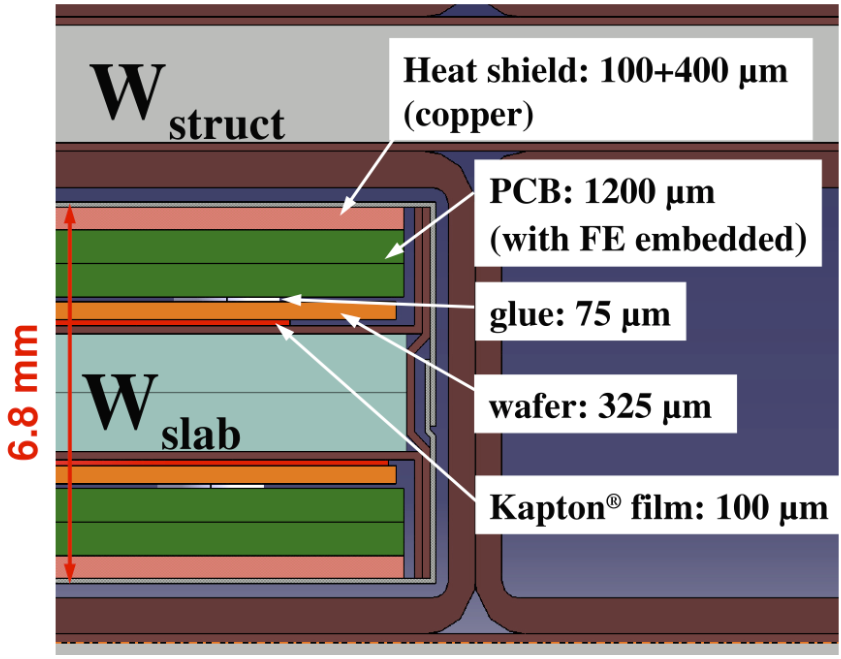
\includegraphics[width=0.4\textwidth]{LCDetectorsAndPFlow/Plots/Pictures/SiECal.png}} 
\hspace{1cm}
\subfloat[]{\label{fig:ecal2}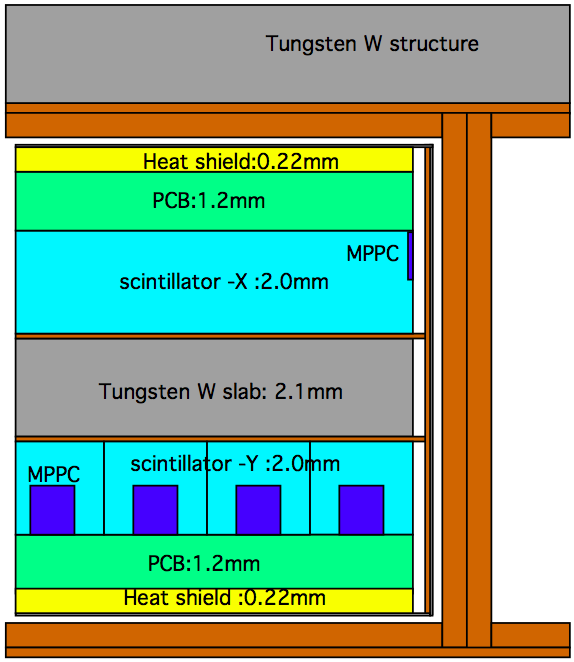
\includegraphics[width=0.4\textwidth]{LCDetectorsAndPFlow/Plots/Pictures/ScECal.png}}
\caption[Cross section through ECal layer for \protect\subref{fig:ecal1} silicon and \protect\subref{fig:ecal2} scintillator option.  Figures taken from  \cite{Behnke:2013lya}.]{Cross section through ECal layer for \protect\subref{fig:ecal1} silicon and \protect\subref{fig:ecal2} scintillator option.  Figures taken from  \cite{Behnke:2013lya}.}
\label{fig:ecal}
\end{figure} 

%========================================================================================

\subsection{Hadronic Calorimeter}
A finely segmented hadronic calorimeter (HCal) surrounds the ECal and its primary goal is the measurement of energy deposits from charged and neutral hadrons.  The focus of the HCal is split between resolving nearby particle showers and measuring their energy analogously to the ECal.  The nominal ILD HCal is a scintillator steel sampling calorimeter containing 48 layers and square cells with a side length of 30 mm.  
 
Steel is used as the absorber material for the HCal as it has durable mechanical properties that allow the HCal to be constructed without the need of auxiliary supports.  If required, auxiliary supports would create dead regions in the detector that would harm performance and so negating the need for them is highly desirable.  Furthermore, steel is relatively inexpensive and it has a small the nuclear interaction length meaning it is possible to achieve a compact calorimeter design at low cost.  The short radiation length found in steel is useful for fine sampling of the electromagnetic shower core that is found in hadronic showers.  This electromagnetic core originates from the creation and decay into {\gamma}s of $\pi^{0}$ and $\eta$ mesons within the hadronic shower.  This fine sampling leads to good energy resolution in the HCal for these shower components.  The nominal ILD HCal contains approximately $6 \lambda_{I}$, which when combined with the $1 \lambda_{I}$ in the ECal is enough to contain the majority of hadronic showers at ILC like energies.  Each of the 48 layers are comprised of 20 mm of steel absorber with a 3 mm scintillator active medium.  The use of square cells with a side length of 30 mm is a balance between reducing the cost of the detector, which is proportional to the number of readout channels, and achieving the required spatial resolution to make particle flow calorimetry possible.  The segmentation of the ILD HCal gives excellent spatial resolution and sufficiently good energy resolution to make the use of particle flow calorimetry a reality.  An optimisation study of the various HCal parameters for the ILD detector can be found in section \ref{sec:hcal}.

Simulation of the ILD HCal have a number of realistic features included such as detailed modelling of the electronics, detector gaps and the implementation of Birk's law for the scintillator sensitive detector elements.

%========================================================================================

\subsection{Muon Chamber}
The ILD outer detector surrounds the HCal and is comprised of a coil, which generates a 3.5 T magnetic field, followed by an iron yoke.  The magnetic field produced by the coil is crucial for bending charged particles so that their momentum can be determined from the curvature of the path they transverse.  Furthermore, the bending of charged particles leads to greater separation of calorimetric energy deposits between charged and neutral particles, which will reduce the effects of confusion when using particle flow calorimetry.  The yoke is an iron scintillator sampling calorimeter, which consists of 10 layers spaced 140 mm apart followed by 2 (3) layers spaced 600 mm apart for the barrel (endcap) region of the detector as shown in figure \ref{fig:muon}.  There is also an additional sensitive layer for the barrel region placed immediately outside the HCal to help with association energy deposits between the calorimeters and the yoke.  

\begin{figure}[h!]
\centering
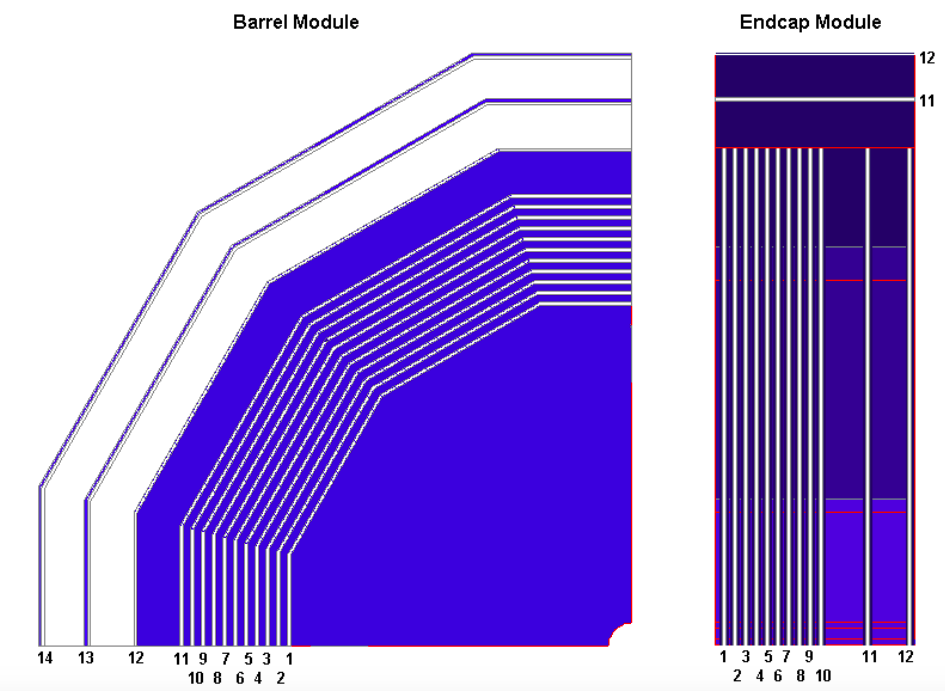
\includegraphics[width=0.5\textwidth]{LCDetectorsAndPFlow/Plots/Pictures/Muon.png}
\caption[The sensitive layers of the ILD muon system.  Figure taken from  \cite{Behnke:2013lya}.]{The sensitive layers of the ILD muon system.  Figure taken from  \cite{Behnke:2013lya}.}
\label{fig:muon}
\end{figure}   

The coil is one of the major cost drivers for the ILD detector and to minimise the size it does not encompass the iron yoke.  The yoke supplements measurements in the calorimeters by acting as a tail catcher for energy leaking out of the calorimeters and, furthermore, is used in the identification of muons.  Iron is used for the yoke absorber material to return the large magnetic flux produced by the coil.  As the majority of particles at ILC like energies will be contained within the calorimeters, the energy and spatial resolution of the yoke are not critical to performance.  It is for that reason that the number of layers is lower and the layer thicknesses wider in the yoke than in the calorimeters.  The nominal ILD model uses 30 mm wide and 1 m long scintillator strips as the readout technology for the yoke.

In the simulation of the ILD yoke a square cell size of 30 mm is assumed.  This is in contrast to the nominal ILD model, but as the tail-catcher plays a minimal role in event reconstruction at ILC like energies this difference should have negligible impact.  

%========================================================================================

\subsection{Forward Calorimetry}
Three additional sampling calorimeters are envisaged for the linear collider experiment: the, LumiCal, the LHCal and the BeamCal.  Their purpose is to extend the coverage of the detector towards 4\pi and monitor the beam quality.  The LumiCal will aim to measure the luminosity with a precision of less than $10^{-3}$ at 500 GeV using Bhabha scattering, $\text{e}^{+}\text{e}^{-} \rightarrow \text{e}^{+}\text{e}^{-}(\gamma)$, as a gauge process \cite{Abe:2010aa}.  The BeamCal will make a bunch-bunch estimate of the luminosity and assist in the beam tuning.  Alongside the LumiCal is the LHCal, which extends the coverage of the HCal to low polar angle as shown in figure \ref{fig:fcal}.  The LumiCal covers polar angles between 31 and 77 mrad, while the BeamCal covers the range between 5 and 40 mrad.  The presence of beam-induced backgrounds along the beam line means these calorimeters will have to be radiation hard.  
 
\begin{figure}[h!]
\centering
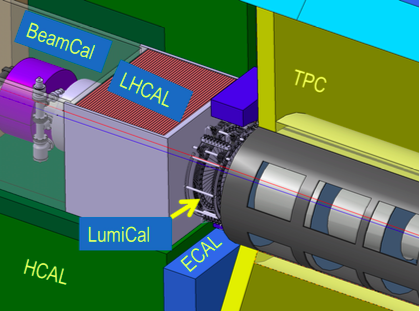
\includegraphics[width=0.5\textwidth]{LCDetectorsAndPFlow/Plots/Pictures/FCal.png}
\caption[The very forward revion of the ILD detector.  LumiCal, BeamCal and LHCal are carried by the support tube for the final focusing quadruple, QD0, and the beam pipe.  Figure taken from  \cite{Behnke:2013lya}.]{The very forward revion of the ILD detector.  LumiCal, BeamCal and LHCal are carried by the support tube for the final focusing quadruple, QD0, and the beam pipe.  Figure taken from  \cite{Behnke:2013lya}.}
\label{fig:fcal}
\end{figure} 

As the primary focus of these calorimeters is measuring the $\text{e}^{+}\text{e}^{-}$  beam, they are all constructed using tungsten absorber material to ensure narrow electromagnetic showers form within them.  The LumiCal layer configuration mirrors that of the ECal giving it a total of $\approx 24 X_{0}$ across its 30 layers.  Silicon is used as sensitive detector element for the LumiCal.  The LHCal uses silicon readout sensors identical to those found in the LumiCal and in total the LHCal contains $4 \lambda_{I}$ across 40 layers.  The BeamCal sensitive detector material is currently being developed as, due to the high occupancy from the beam induced backgrounds, a fast readout is required.  The cell sizes for these calorimeters is yet to be confirmed.  

These calorimeters play a minimal role in event reconstruction as few particles from the hard physics interaction will have their energy measured by these calorimeters.  It is for this reason that they are not used in the simulation.


%========================================================================================

\section{Simulation}

%========================================================================================

\section{CLIC ILD}
The increased collision energy found at the CLIC experiment mean the use of the nominal ILD detector model would be inappropriate.  Therefore, a new detector model, CLIC\_ILD \cite{Linssen:2012hp}, based upon the nominal ILD detector model was created to cope with the experimental conditions found at the CLIC experiment.  Several modifications were made to the nominal ILD detector model to make it more suitable for the CLIC experiment.  The key differences between the nominal ILD detector and CLIC\_ILD are:

\begin{figure}[h!]
\centering
\subfloat[]{\label{fig:clicild1}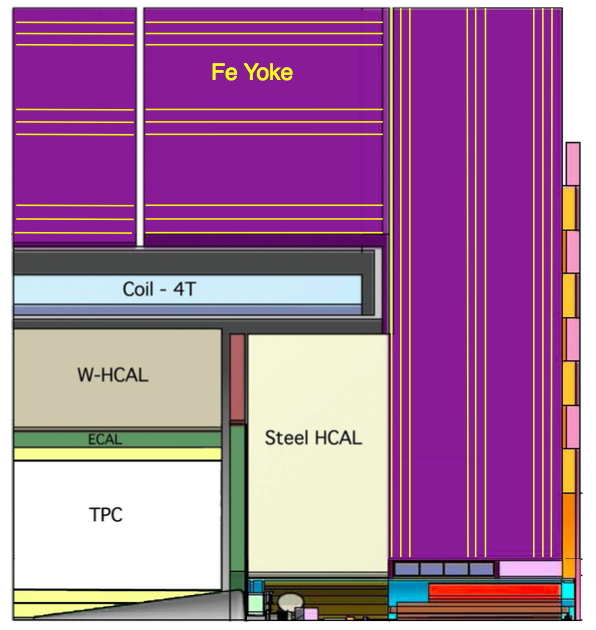
\includegraphics[width=0.4\textwidth]{LCDetectorsAndPFlow/Plots/Pictures/CLIC_ILD.png}}
\hspace{1cm}
\subfloat[]{\label{fig:clicild2}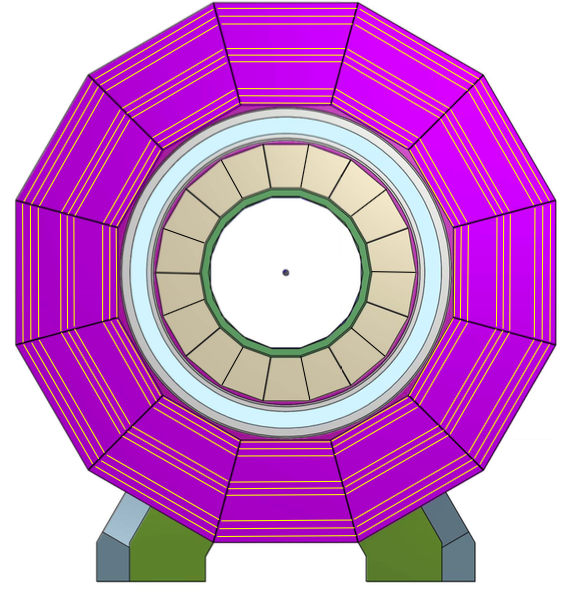
\includegraphics[width=0.4\textwidth]{LCDetectorsAndPFlow/Plots/Pictures/CLIC_ILD_2.png}}
\caption[\protect\subref{fig:ild1} Longitudinal (top quadrant) and \protect\subref{fig:ild2} transverse cross section of the CLIC\_ILD detector.  Figures taken from \cite{Linssen:2012hp}.]{\protect\subref{fig:ild1} Longitudinal (top quadrant) and \protect\subref{fig:ild2} transverse cross section of the CLIC\_ILD detector.  Figures taken from \cite{Linssen:2012hp}.}
\label{fig:clicild}
\end{figure} 

\begin{itemize}
\item The higher energies found at the CLIC experiment lead to more intense beam induced backgrounds, which is especially problematic for detectors close to the IP where the occupancies will be extremely high.  To attempt to compensate for these effects the inner vertex detector in CLIC\_ILD is moved 15 mm further out from the IP.    
\item The HCal thickness is increased from 6 $\lambda_{I}$ to 7.5 $\lambda_{I}$.  This ensures that higher energy particle showers found at the CLIC experiment are in general contained within the calorimeters.  
\item The HCal absorber material for the barrel is tungsten as opposed to steel.  This reduces the overall thickness of the HCal and keeps the coil size, one of the driving cost factors for the detectors, similar for the nominal ILD and CLIC\_ILD detectors.  In the endcaps steel is used as the absorber material as there are no spatial requirements relating to the coil size and this will lower the detector cost.  Furthermore, the shower development time in steel is faster than in tungsten making effective time stamping of energy deposits easier, which is crucial for the CLIC experiment for vetoing beam induced backgrounds.  
\item The magnetic field strength in the CLIC\_ILD detector is increased to 4 T.  This was found to benefit the reconstruction, particularly at high energies, as it leads to greater separation of charged particle tracks.  Furthermore, it was possible to achieve this increase in field strength using the nominal ILD coil design.   
\end{itemize}  

%========================================================================================

%%%%%%% This is new!

\subsection{Experimental Conditions at CLIC}

The CLIC experiment will operate in a unique environment in comparison to previous generations of lepton colliders and this must be properly accounted for to get an accourate measure of the physics potential that CLIC has to offer.  The following aspects of the CLIC experiment present the largest challenges to the physics potential for the CLIC experiment:

\begin{itemize}
\item The high bunch charge density.  The small beam size at the impact point produces very large electromagnetic fields.  These fields can interact with the opposite beam particles causing them to radiate photons in an effect known as beamstrahlung.  Beamstrahlung acts to reduce the collision energy of the $\text{e}^{+}\text{e}^{-}$ pairs.   
\item Beam related backgrounds.  Beamstrahlung photons can subsequently interact to produce background events that must be accounted for.  Dominant backgrounds of this form that cannot be easily vetoed in the reconstruction include incoherent pair production of $\text{e}^{+}\text{e}^{-}$ and $\gamma\gamma \rightarrow \text{Hadron}$.  
\item Fast readout technology is crucial.  The CLIC bunch train consists of 312 bunches with a repetition rate of 50 Hz.  Each bunch is separated by 0.5ns, therefore, it will be necessary to integrate over multiple bunch crossing when reading out the detectors.  This places tight constraints on all detector electrical readout speeds and time resolutions.   
\end{itemize}

\subsubsection{Beam-Related Backgrounds at CLIC}
The primary sources of background for the CLIC experiment are as follows:
\begin{itemize}
\item $\text{e}^{+}\text{e}^{-}$ pair creation from the interaction of a beamstrahlung photons with the opposing beam.  The different mechanisms for pair creation are as follows:
\begin{itemize}
\item \textbf{Coherent pair production}.  This mechanism involves the interaction of a real beamstrahlung photon with the electromagnetic field from the opposing beam.
\item \textbf{Trident pair production}.  This mechanism involves the interaction of a virtual beamstrahlung photon with the electromagnetic field from the opposing beam.
\item \textbf{Incoherent pair production}.  This mechanism involves the interaction of a real or virtual beamstrahlung photon with the individual particles in the opposing beam.
\end{itemize}
\item $\gamma\gamma \rightarrow \text{Hadron}$ from the interaction of real or virtual beamstrahlung photons with each other.  Example Feynman diagrams for such processes is shown in figure ??. 
\item Beam halo muons that arise from interactions of the beam particles during collimation.  The dominant mechanisms producing beam halo muons are photon conversions into muon pairs ($\gamma \text{e}^{-} \rightarrow \mu^{+}\mu^{-}\text{e}^{-}$) and annihilation of positrons with atomic $\text{e}^{-}$ into muon pairs ($\text{e}^{+}\text{e}^{-} \rightarrow \mu^{+}\mu^{-}$) \cite{Pilicer:2015ijy}.
\end{itemize}

Each of these has to be properly addressed to get a true measure of the physics potential at CLIC.  Coherent and trident pair production is not a dominant source of background as they are produced at low transverse momenta, as figure \ref{fig:backgroundangle} shows, and a simple cut would veto these backgrounds.  This is not the case for incoherent pair production of $\text{e}^{+}\text{e}^{-}$, which are dominant in the forward regions of the detector, and $\gamma\gamma \rightarrow \text{Hadron}$, which are dominant in the tracker and the calorimeters (with the exception of low radii in the calorimeter endcaps) \cite{Linssen:2012hp, Sailer:2012mfa}.  Beam halo muons are not a major source of background either as they can be easily removed during the reconstruction due to the clear signal they create in the detector.  An algorithm was developed within the PandoraPFA framework for this purpose and it was found to be highly effective at removing the beam halo muons background \cite{Linssen:2012hp}.  

$\gamma\gamma \rightarrow \text{Hadron}$ events are the most dominant source of background to consider at CLIC as these events deposit more energy throughout the detector than incoherent pair production of $\text{e}^{+}\text{e}^{-}$ events \cite{Linssen:2012hp}.  The effect of the $\gamma\gamma \rightarrow \text{Hadron}$ background is incorporated into this analysis by overlaying $\gamma\gamma \rightarrow \text{Hadron}$ events onto the event samples used in this analysis.  The overlaid backgrounds are added prior to reconstruction so that their effect on the reconstruction is fully accounted for.  For a given event the exact number of background events overlaid is drawn from a Poisson distribution with a mean of 3.2 (1.3) events per bunch crossing at 3 (1.4) TeV.  While incoherent pairs are still a source of background they will produce a second order effect in comparison to the $\gamma\gamma \rightarrow \text{Hadron}$ events.

The PFO choices described in section \ref{sec:optimisationjetalgo} are applied to veto the effect of PFOs that arise from the overlaid $\gamma\gamma \rightarrow \text{Hadron}$ events.

\begin{figure}
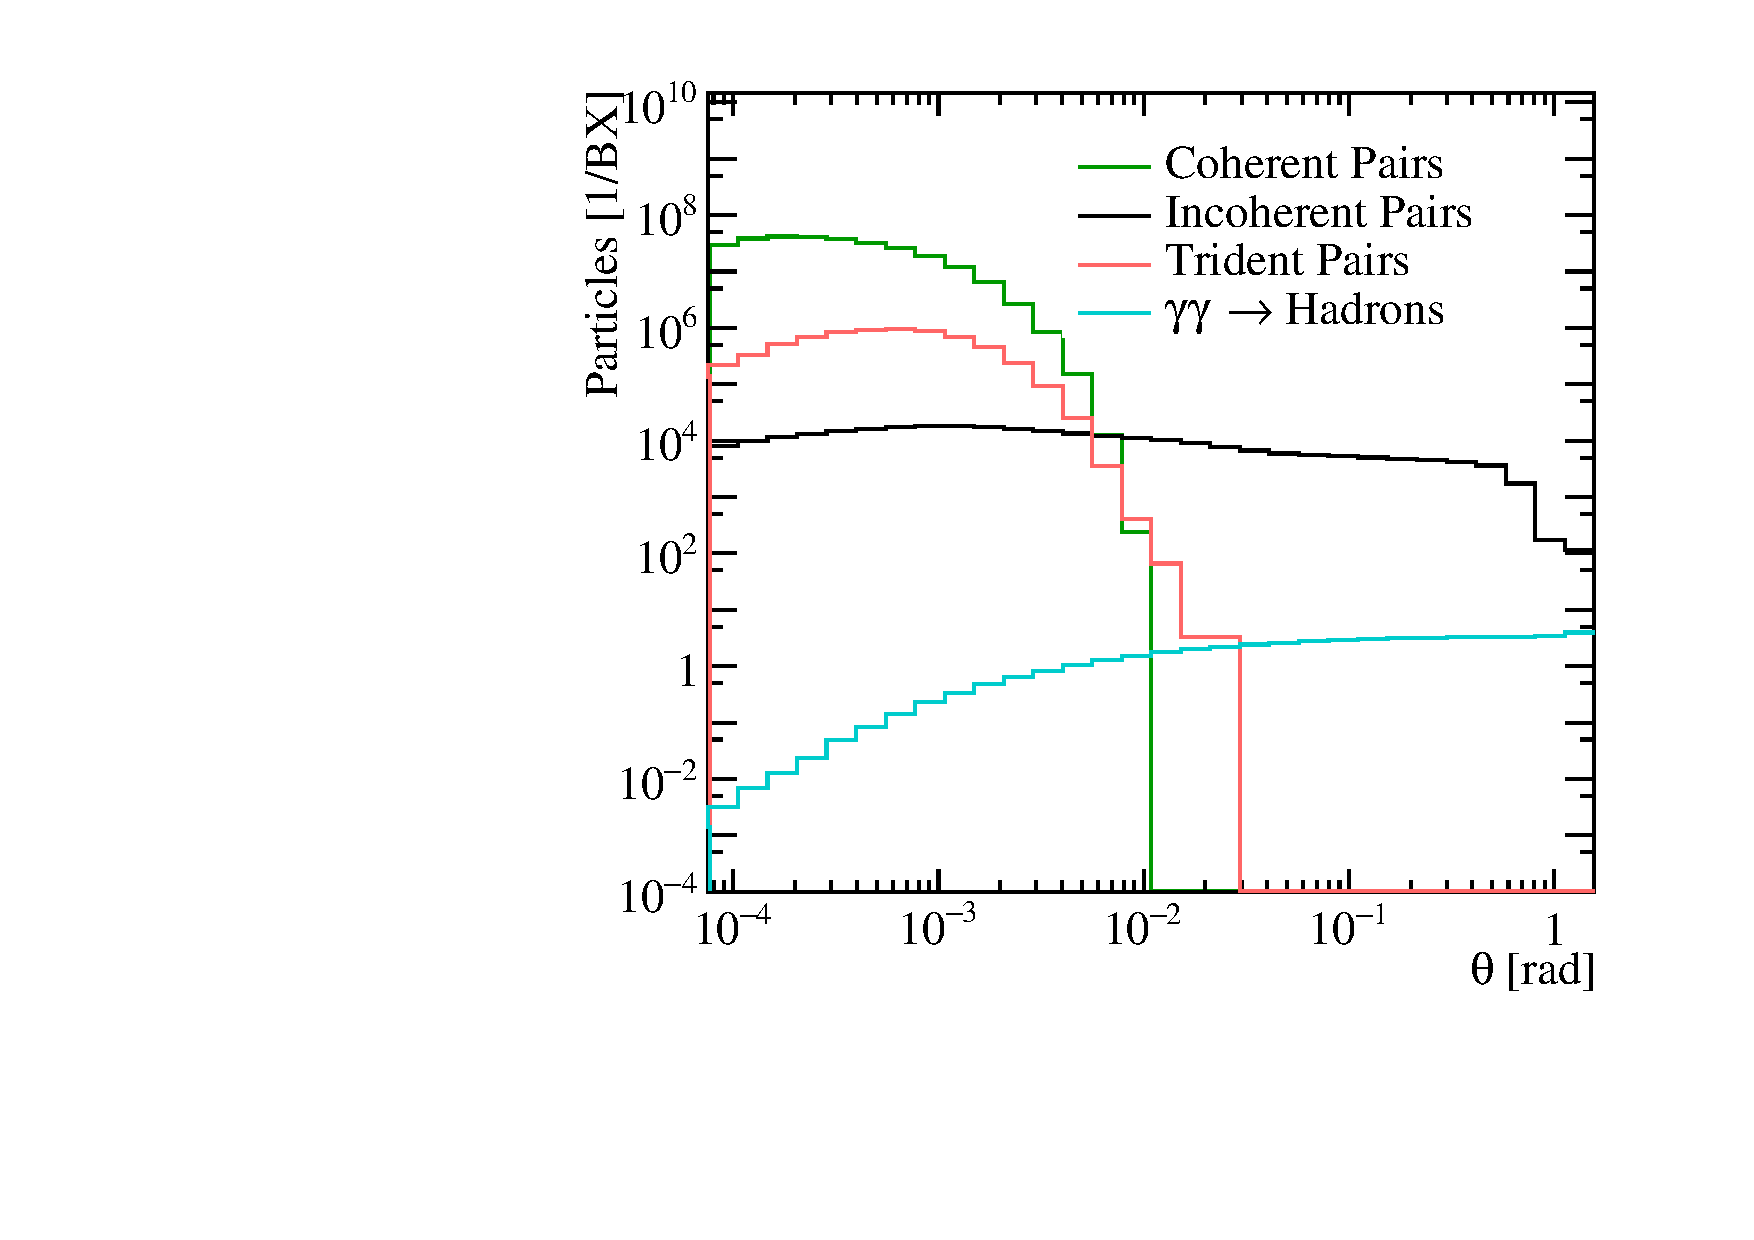
\includegraphics[width=0.5\textwidth]{FutureLinearColliders/Plots/CDRPlots/BackgroundAngleCut.pdf}
\caption[]{Angular distribution of number of particles for beam induced backgrounds for CLIC at $\sqrt{s} = 3$ TeV.  Taken from CLIC CDR.}
\label{fig:backgroundangle}
\end{figure}

%========================================================================================
%======================================================================================== 

\section{Particle Flow Reconstruction}
Particle flow calorimetry relies upon correct associations being made between calorimetric energy deposits and charged particle tracks.  Even with a finely segmented detector, such as the ILD detector described in section \ref{sec:ild}, correctly making these associations is a highly a non-trivial task and must be done using advanced pattern recognition software.  This is provided by the PandoraPFA particle flow algorithm \cite{arXiv:0907.3577, arXiv:1209.4039}.

%======================================================================================== 

\subsection{PandoraPFA}
PandoraPFA applies the pattern recognition logic in eight main stages:
\begin{enumerate}
\item Track selection.  The input track collections are examined to determine whether $V^{0}$ decays, two charged tracks originating from a point displaced from the IP, or kinks, where a charged particle has decayed into a single charged particle and a number of neutral ones, are present.  Such information will be propagated in the reconstruction to the final PFO creation stage.  
\item Calorimeter hit selection.  This stage is broken down into several steps:
\begin{itemize}
\item The various collection of, post digitisation, calorimeter hits are passed into the Pandora framework and converted into Pandora calorimeter hits.  These objects are self describing so that the Pandora pattern recognition logic has no dependancy on the external software framework.  
\item A minimum ionising particle equivalent energy cut is applied to the calorimeter hits.  If a calorimeter hit contains less than 0.5 (0.3) of the energy of a normally incident MIP passing through the calorimeter cell in the ECal (HCal) then it is not used in the reconstruction.  
\item Calibration of the energy contained within the calorimeter hits is flagged up at this point, however, it is not directly applied at this stage.  The energy contribution for each calorimeter cell ultimately depends on whether the associated cluster of calorimeter hits is deemed to originate from an electromagnetic or hadronic shower.  Different scale factors are applied to the energy for electromagnetic and hadronic showers to account for effects such as the invisible energy component in hadronic showers.  These energy factors are used throughout the reconstruction, including the final reconstructed particle energy, once the particle shower type has been identified.  For energy comparisons prior to the shower type being identified the uncorrected calorimeter hit energy is used.  Further details on how these calibration constants are determined can be found in section \ref{sec:calibration}.  
\item To minimise any dependancy on the detector geometry each calorimeter hit is assigned to a pseudo-layer, which is representative of the calorimeter stave layer.  All further topological association algorithms work using the pseudo-layer definition, illustrated in figure \ref{fig:pseudolayer}.  
\item If a calorimeter hit is sufficiently far away from other hits, it is flagged as an isolated hit.  Such hits are most likely due to low energy neutrons produced in hadronic showers, which can travel a significant distance from the original shower before depositing energy.  Due to the distance they travel these hits are very difficult to associate to the correct particle shower.  Furthermore, as such hits are unlikely to be the seed for a particle shower they are not used by the initial clustering algorithm.  
\item Any calorimeter hit that contains an energy consistent with a MIP signal and where, at most, one Pandora calorimeter hit exists in the neighbouring cells within the same layer is flagged as a MIP consistent hit.  This information is used in the identification of MIPs in the reconstruction.
\end{itemize}
\item Clustering.  This begins by using the projection of the charged particle tracks onto the front face of the ECal as seeds for the initial clustering phase.  Calorimeter hits are looped over on a per layer basis, working from the inner to the outer pseudo-layer, and if they fall within a cone of fixed dimensions surrounding a cluster direction they are associated to the cluster.  If no association can be made to any preexisting calorimeter hit clusters then the calorimeter hit is used to seed a new cluster.  
\item Topological cluster merging.  The initial clustering algorithm is designed to be conservative to avoid mixing together energy deposits from several particles.  The fragments produced by the initial clustering are then merged together by various algorithms whose logic is motivated by a number of well-motivated topological rules, such as those shown figure \ref{fig:associations}.  
\item Statistical re-clustering.  Comparisons between the cluster energy and any associated track momenta are made to determine whether they are consistent.  If a large discrepancy is observed then statistical re-clustering is initiated.  This involves running a number of differently configured algorithms to change the cluster configuration to determine if a new optimal configuration of tracks and clusters can be found.  
\item Photon identification and recovery.  Topological likelihood data is used to identify clusters of calorimeter hits that are consistent with $\gamma$s.  This is possible due to the clear transverse and longitudinal profiles observed for electromagnetic showers.  
\item Fragment removal.  Neutral clusters originating from a nearby charged particle cluster are identified and merged back into the parent charged particle cluster.  These algorithms take into account the changes in the compatibility of the track and cluster associations when merging any neutral clusters into charged clusters.  
\item Formation of particle flow objects.  Finally, reconstructed particles are produced.  The energy for charged particles is taken from the track momenta, while neutral particle energies are taken from the calorimeter cluster measurements.  Furthermore, the different electromagnetic and hadronic scales are applied to the output neutral particle energies depending on whether the neutral cluster is consistent with a $\gamma$.  
\end{enumerate}

\begin{figure}[h!]
\centering
\subfloat[]{\label{fig:pseudolayer1}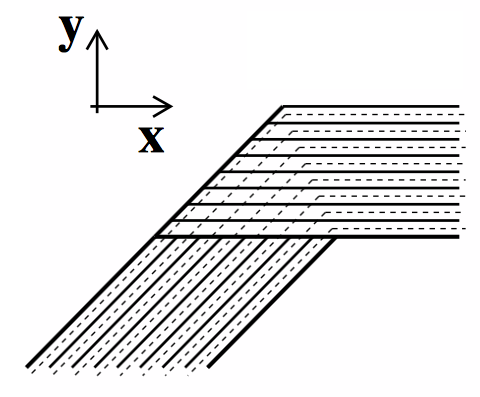
\includegraphics[width=0.4\textwidth]{LCDetectorsAndPFlow/Plots/Pictures/PseudoLayer1.png}}
\hspace{1cm}
\subfloat[]{\label{fig:pseudolayer2}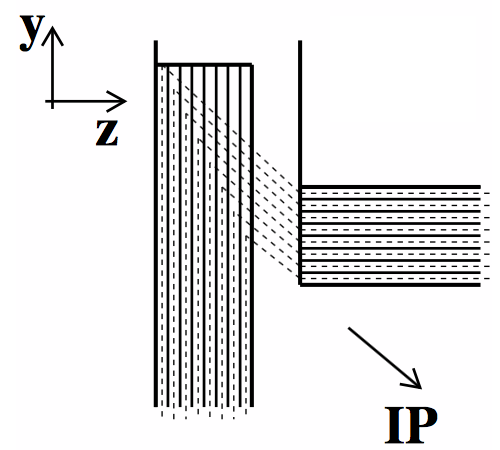
\includegraphics[width=0.4\textwidth]{LCDetectorsAndPFlow/Plots/Pictures/PseudoLayer2.png}}
\caption[Schematic showing the definition of the pseudo-layer assignment for calorimeter hits.  The solid lines indicate the positions of the physics ECal layers and the dashed lines show the definition of the virtual pseudo-layers.  \protect\subref{fig:pseudolayer1} The $xy$-view showing the ILD ECal stave structure.  \protect\subref{fig:pseudolayer2} The $xz$ view showing a possible layout for the ECal barrel/endcap overlap region.  The pseudo-layers are defined using projection back to the IP.  Figures taken from \cite{arXiv:0907.3577}.]{Schematic showing the definition of the pseudo-layer assignment for calorimeter hits.  The solid lines indicate the positions of the physics ECal layers and the dashed lines show the definition of the virtual pseudo-layers.  \protect\subref{fig:pseudolayer1} The $xy$-view showing the ILD ECal stave structure.  \protect\subref{fig:pseudolayer2} The $xz$ view showing a possible layout for the ECal barrel/endcap overlap region.  The pseudo-layers are defined using projection back to the IP.  Figures taken from \cite{arXiv:0907.3577}.}
\label{fig:pseudolayer}
\end{figure} 

\begin{figure}[h!]
\centering
\subfloat[]{\label{fig:association1}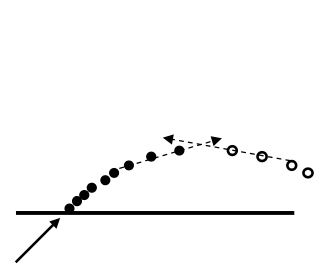
\includegraphics[width=0.2\textwidth]{LCDetectorsAndPFlow/Plots/Pictures/Association1.png}}
\hspace{5mm}
\subfloat[]{\label{fig:association2}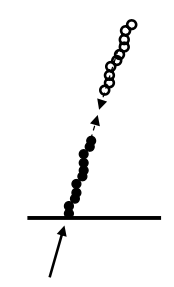
\includegraphics[width=0.2\textwidth]{LCDetectorsAndPFlow/Plots/Pictures/Association2.png}}
\hspace{5mm}
\subfloat[]{\label{fig:association3}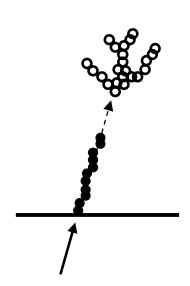
\includegraphics[width=0.2\textwidth]{LCDetectorsAndPFlow/Plots/Pictures/Association3.png}}
\hspace{5mm}
\subfloat[]{\label{fig:association4}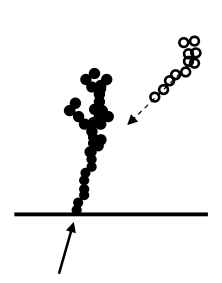
\includegraphics[width=0.2\textwidth]{LCDetectorsAndPFlow/Plots/Pictures/Association4.png}} \\
\subfloat[]{\label{fig:association5}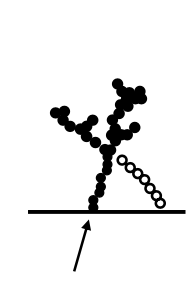
\includegraphics[width=0.2\textwidth]{LCDetectorsAndPFlow/Plots/Pictures/Association5.png}}
\hspace{5mm}
\subfloat[]{\label{fig:association6}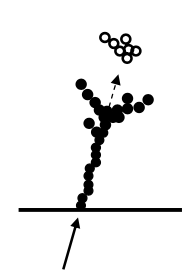
\includegraphics[width=0.2\textwidth]{LCDetectorsAndPFlow/Plots/Pictures/Association6.png}}
\hspace{5mm}
\subfloat[]{\label{fig:association7}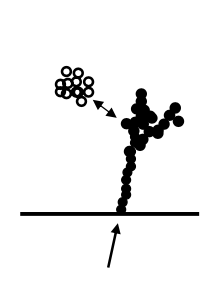
\includegraphics[width=0.2\textwidth]{LCDetectorsAndPFlow/Plots/Pictures/Association7.png}}
\hspace{5mm}
\subfloat[]{\label{fig:association8}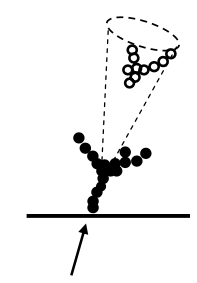
\includegraphics[width=0.2\textwidth]{LCDetectorsAndPFlow/Plots/Pictures/Association8.png}}
\hspace{5mm}
\subfloat[]{\label{fig:association9}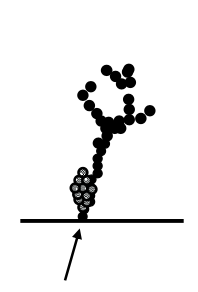
\includegraphics[width=0.2\textwidth]{LCDetectorsAndPFlow/Plots/Pictures/Association9.png}}
\caption[The main topological rules for cluster merging: \protect\subref{fig:association1} looping track segments; \protect\subref{fig:association2} track segments with gaps; \protect\subref{fig:association3} track segments pointing to hadronic showers; \protect\subref{fig:association4} track-like neutral clusters pointing back to a hadronic shower; \protect\subref{fig:association5} back-scattered tracks from hadronic showers; \protect\subref{fig:association6} neutral clusters which are close to a charged cluster; \protect\subref{fig:association7} a neutral cluster near a charged cluster; \protect\subref{fig:association8} cone association; and \protect\subref{fig:association9} recover of photons which overlap with a track segment.  In each case the arrow indicates the track, the filled points represent the hits in the associated cluster and the open points represent hits in the neutral cluster.  Figures taken from \cite{arXiv:0907.3577}.]{The main topological rules for cluster merging: \protect\subref{fig:association1} looping track segments; \protect\subref{fig:association2} track segments with gaps; \protect\subref{fig:association3} track segments pointing to hadronic showers; \protect\subref{fig:association4} track-like neutral clusters pointing back to a hadronic shower; \protect\subref{fig:association5} back-scattered tracks from hadronic showers; \protect\subref{fig:association6} neutral clusters which are close to a charged cluster; \protect\subref{fig:association7} a neutral cluster near a charged cluster; \protect\subref{fig:association8} cone association; and \protect\subref{fig:association9} recover of photons which overlap with a track segment.  In each case the arrow indicates the track, the filled points represent the hits in the associated cluster and the open points represent hits in the neutral cluster.  Figures taken from \cite{arXiv:0907.3577}.}
\label{fig:associations}
\end{figure} 

The application of the pattern recognition algorithms in PandoraPFA when combined with a highly segmented detector make particle flow calorimetry a reality.  In turn this provides excellent jet energy resolution for studying many interesting physics processes at the linear collider experiment.

%======================================================================================== 

\subsection{Performance}



